\documentclass{article}
\usepackage{tikz}
\usetikzlibrary{arrows.meta}
\usepackage{mathtools}
\usepackage{amsmath}
\usepackage{amssymb}
\usepackage{amsfonts}
\usepackage{graphicx}
\usepackage{float}
\usepackage{multirow}
\usepackage{verbatim}
\usepackage{listings}

\linespread{1.3}
\setlength{\parindent}{0em}
\setlength{\parskip}{1em}
\setcounter{secnumdepth}{0}
\setcounter{MaxMatrixCols}{20}
\renewcommand{\arraystretch}{1.5}

\newcommand{\ts}{\textsuperscript}
\newcommand{\diff}{\mathop{}\!\mathrm{d}}
\newcommand{\prob}{\mathbb{P}}
\newcommand{\expect}{\mathbb{E}}
\newcommand{\var}{\text{Var}}

\DeclarePairedDelimiter{\abs}{\lvert}{\rvert}
\DeclarePairedDelimiter\norm{\lVert}{\rVert}
\DeclarePairedDelimiter\p{\lparan}{\rparan}

\title{STAT3004 Assignment 3}
\author{Joshua Hwang (44302650)}

\begin{document}
\section{1}
\subsection{a}
By drawing the Markov chain we reveal our possible transitions.

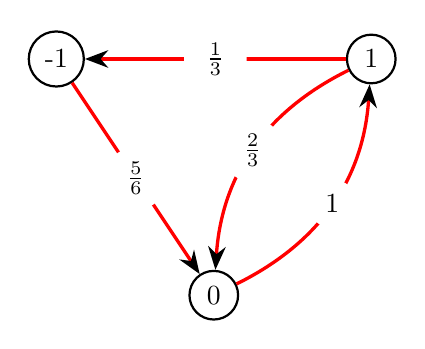
\begin{tikzpicture}
    \begin{scope} [every node/.style={circle,thick,draw}]
        \node (-1) at (0,0) {-1};
        \node (0) at (2,-3) {0};
        \node (1) at (4,0) {1};
    \end{scope}

    \begin{scope}[>={Stealth[black]},
            every node/.style={fill=white,circle},
            every edge/.style={draw=red,very thick}]
        \path [->] (-1) edge node {$\frac{5}{6}$} (0);
        \path [->] (1) edge node {$\frac{1}{3}$} (-1);
        \path [->] (0) edge[bend right=30] node {$1$} (1);
        \path [->] (1) edge[bend right=30] node {$\frac{2}{3}$} (0);
    \end{scope}
\end{tikzpicture}

We note that if $X_0 = 0$ then there is no way to get $X_2 = 1$ thus \\
$\prob(X_2 = 1 | X_0 = 0) = 0$.

We now use this same technique to determine $\prob(X_2 = 1)$,
\begin{align*}
    \prob(X_2 = 1) &= \prob(X_2 = 1 | X_0 = 0) \prob(X_0 = 0) \\
                   &+ \prob(X_2 = 1 | X_0 = 1) \prob(X_0 = 1) \\
                   &+ \prob(X_2 = 1 | X_0 = -1) \prob(X_0 = -1) \\
    \prob(X_2 = 1) &= 0 \times \prob(X_0 = 0) \\
                   &+ \frac{2}{3} \prob(X_0 = 1) \\
                   &+ \frac{5}{6} \prob(X_0 = -1) \\
    \prob(X_2 = 1) &= \frac{2}{3} \times \frac{1}{2}
                    + \frac{5}{6} \times \frac{1}{6} \\
    \prob(X_2 = 1) &= \frac{1}{3} + \frac{5}{36} \\
    \prob(X_2 = 1) &= \frac{17}{36} \\
\end{align*}

\subsection{b}
To get the expectation we need to repeat this process for $\prob(X_2 = -1)$
and $\prob(X_2 = 0)$.
\begin{align*}
    \prob(X_2 = -1) &= \prob(X_2 = -1 | X_0 = 0) \prob(X_0 = 0) \\
                    &+ \prob(X_2 = -1 | X_0 = 1) \prob(X_0 = 1) \\
                    &+ \prob(X_2 = -1 | X_0 = -1) \prob(X_0 = -1) \\
    \prob(X_2 = -1) &= \frac{1}{3} \prob(X_0 = 0) \\
                    &+ \frac{1}{3} \times \prob{1}{6} \prob(X_0 = 1) \\
                    &+ \frac{1}{6} \times \frac{1}{6} \prob(X_0 = -1) \\
    \prob(X_2 = -1) &= \frac{1}{3} \times \frac{1}{3} \\
                    &+ \frac{1}{18} \times \frac{1}{2} \\
                    &+ \frac{1}{36} \times \frac{1}{6} \\
    \prob(X_2 = -1) &= \frac{31}{216}
\end{align*}
\begin{align*}
    \prob(X_2 = 0) &= \prob(X_2 = 0 | X_0 = 0) \prob(X_0 = 0) \\
                   &+ \prob(X_2 = 0 | X_0 = 1) \prob(X_0 = 1) \\
                   &+ \prob(X_2 = 0 | X_0 = -1) \prob(X_0 = -1) \\
    \prob(X_2 = 0) &= \frac{83}{216}
\end{align*}

We can now determine $\expect[X]$ and $\expect[X^2]$.
\begin{align*}
    \expect[X_2]&= 0 \times \prob(X_2 = 0) + \prob(X_2 = 1) - \prob(X_2 = -1) \\
                &= \frac{17}{36} - \frac{31}{216} \\
                &= \frac{71}{216} \\
\end{align*}

\begin{align*}
    \expect[X_2^2] &= 0 \times \prob(X_2 = 0)
                    + \prob(X_2 = 1) + \prob(X_2 = -1) \\
                   &= \frac{17}{36} + \frac{31}{216} \\
                   &= \frac{133}{216} \\
\end{align*}

\begin{align*}
    \var X_2 &= \expect[X_2^2] - \expect{[X_2]}^2 \\
             &= \frac{133}{216} - {(\frac{71}{216})}^2 \\
             &= \frac{23687}{46656} \\
\end{align*}

Thus, $\expect[X_2] = \frac{71}{216}$ and $\var[X_2] = \frac{23687}{46656}$.

\subsection{c}
A stationary distribution is defined as $\pi P = \pi$.
\begin{align*}
    \begin{bmatrix}
        a & b & c \\
    \end{bmatrix}
    \begin{bmatrix}
        \frac{1}{6} & \frac{5}{6} & 0 \\
                  0 &           0 & 1 \\
        \frac{1}{3} & \frac{2}{3} & 0 \\
    \end{bmatrix}
    &=
    \begin{bmatrix}
        a & b & c \\
    \end{bmatrix}
\end{align*}

From this we get four equations.
\begin{align*}
    a + b + c &= 1 \\
    \frac{1}{6} a + \frac{1}{3} c &= a \\
    \frac{5}{6} a + \frac{2}{3} c &= b \\
    b &= c \\
\end{align*}

Solving these equations gives us only a single solution.
\begin{align*}
    a &= \frac{1}{6} \\
    b &= \frac{5}{12} \\
    c &= \frac{5}{12}
\end{align*}

We diagonalise the matrix $P$ so it becomes easier to raise to powers.
From here we take $S \Lambda^n S^{-1}$ with $n \to \infty$. Out of the three
eigenvalues, $\lambda = -\frac{1}{2}, -\frac{1}{3}, 1$,
we find only one of them is $\geq 1$.

\begin{align*}
    P
    &=
    \begin{bmatrix}
        \frac{5}{2} &  5 & 1 \\
                 -2 & -3 & 1 \\
                  1 &  1 & 1 \\
    \end{bmatrix}
    \begin{bmatrix}
        -\frac{1}{2} &            0 & 0 \\
                   0 & -\frac{1}{3} & 0 \\
                   0 &            0 & 1 \\
    \end{bmatrix}
    \begin{bmatrix}
        -\frac{2}{3} & -\frac{2}{3} & \frac{4}{3} \\
         \frac{1}{2} &  \frac{1}{4} & -\frac{3}{4} \\
         \frac{1}{6} & \frac{5}{12} & \frac{5}{12} \\
    \end{bmatrix} \\
    P^n
    &=
    \begin{bmatrix}
        \frac{5}{2} &  5 & 1 \\
                 -2 & -3 & 1 \\
                  1 &  1 & 1 \\
    \end{bmatrix}
    \begin{bmatrix}
        -\frac{1}{2}^n &              0 & 0 \\
                     0 & -\frac{1}{3}^n & 0 \\
                     0 &              0 & 1^n \\
    \end{bmatrix}
    \begin{bmatrix}
        -\frac{2}{3} & -\frac{2}{3} & \frac{4}{3} \\
         \frac{1}{2} &  \frac{1}{4} & -\frac{3}{4} \\
         \frac{1}{6} & \frac{5}{12} & \frac{5}{12} \\
    \end{bmatrix} \\
    P^n
    &=
    \begin{bmatrix}
        \frac{5}{2} &  5 & 1 \\
                 -2 & -3 & 1 \\
                  1 &  1 & 1 \\
    \end{bmatrix}
    \begin{bmatrix}
        0 & 0 & 0 \\
        0 & 0 & 0 \\
        0 & 0 & 1 \\
    \end{bmatrix}
    \begin{bmatrix}
        -\frac{2}{3} & -\frac{2}{3} & \frac{4}{3} \\
         \frac{1}{2} &  \frac{1}{4} & -\frac{3}{4} \\
         \frac{1}{6} & \frac{5}{12} & \frac{5}{12} \\
    \end{bmatrix} \\
    P^n
    &=
    \begin{bmatrix}
        \frac{1}{6} & \frac{5}{12} & \frac{5}{12} \\
        \frac{1}{6} & \frac{5}{12} & \frac{5}{12} \\
        \frac{1}{6} & \frac{5}{12} & \frac{5}{12} \\
    \end{bmatrix}
\end{align*}

Thus our stationary distribution is our limiting distribution.

\subsection{d}
The code used is below.
\lstinputlisting{q1d.py}

These are the results.
\begin{verbatim}
==================================================
P(X2=1) ~ 0.478
P(X2=1) = 0.4722222222222222
--------------------------------------------------
E[X2] ~ 0.303
E[X2] = 0.3287037037037037
--------------------------------------------------
Var(X2) ~ 0.5617527527527606
Var(X2) = 0.5076946159122085
==================================================
\end{verbatim}

% ZZZ need to include standard errors

\end{document}
